\documentclass[11pt,a4paper]{article}
\usepackage[hyperref]{acl2017}
\usepackage{times}
\usepackage{latexsym}

\usepackage{url}

% New Packages!!
% \usepackage{CJKutf8}

\usepackage{amsmath, amssymb}
\usepackage{bm} % 数学粗体包
\usepackage{tabularx} % 表格增强包
\usepackage{booktabs} % 三线表格包
\usepackage{caption, subcaption} % 图表标题包
\usepackage{multirow} % 表格跨列跨行
\usepackage{graphicx}

\aclfinalcopy % Uncomment this line for the final submission
%\def\aclpaperid{***} %  Enter the acl Paper ID here

%\setlength\titlebox{5cm}
% You can expand the titlebox if you need extra space
% to show all the authors. Please do not make the titlebox
% smaller than 5cm (the original size); we will check this
% in the camera-ready version and ask you to change it back.

\newcommand\BibTeX{B{\sc ib}\TeX}

\title{Report of Douban Movie Recommendation}
%TODO
\author{Jiancong Gao \\
  School of Data Science \\
  Fudan University \\
  Shanghai, China \\
  {\tt 15300180050@fudan.edu.cn} \\\And
  Linyang He \\
  School of Data Sciences \\
  Fudan University \\
  Shanghai, China \\
  {\tt lyhe15@fudan.edu.cn} \\}

\date{}

\begin{document}
\maketitle
\section{Data Visualization}

In this project, we use the \emph{Gephi} application to implement the
Douban user data visualization. Gephi is an open-source network analysis
and visualization software package written in Java on the NetBeans
platform. It was initially developed by students of the University of
Technology of Compiègne in France.

Considering that the whole dataset is quite slow to run the
visualization program, and the whole dataset will not promise a good
visualization result, we randomly extract a subset of the user dataset
with 246 users, and we will count the following users and followers of
this user, which makes the total number of users is 12678. Besides, we
can build an \emph{adjacent matrix} to represent the directed graph. The
following and followed information can be denoted in a directed graph as
the figure showing. In summary, there're 12678 nodes representing the
users and 16144 edges representing the following information. We will
illustrate some important information the graph can tell.

\subsection{Pointed Edge}

The single pointed arrow between \(U_2\) and \(U_1\) suggests that
\(U_2\) follows \(U_1\) but \(U_1\) does not follow \(U_1\). Also, the
double pointed arrow between \(U_1\) and \(U_3\) means that these two
users follow each other.

\begin{figure}
\centering
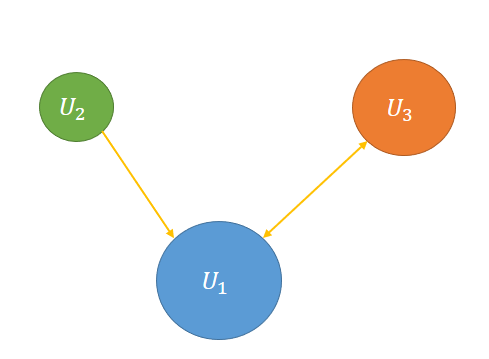
\includegraphics[width = \columnwidth]{1.png}
\caption{}
\end{figure}

\hypertarget{header-n13}{%
\subsection{Node Size}\label{header-n13}}

As you can see from the figure, the sizes of these three nodes are
different. We use the size information to denote the \emph{In-Degree}
rather than just degree. In this situation, users with more fans or
followers can have a big size.

\hypertarget{header-n16}{%
\subsection{Node Color}\label{header-n16}}

In this project, a quite meaningful feature of the visualization is the
color. We are not coloring the nodes randomly, in contrast, we use
different colors to represent different communities. That is, we
implement a community division algorithm through the data visualization.
We introduce the Fast Unfolding algorithm to make it. Before we
demonstrate the algorithm, we will first introduce the Community
Division task.

\hypertarget{header-n19}{%
\paragraph{Community Division}\label{header-n19}}

The main goal of the community division is to make the connection in the same community more dense while make the connection among different communities more sparse. This can ''split'' the graph into several parts in general based on their following and followed information.

\hypertarget{header-n22}{%
\paragraph{Modularity}\label{header-n22}}

Broadly speaking, modularity is the degree to which a system's
components may be separated and recombined, often with the benefit of
flexibility and variety in use. Modularity is quite an important concept
in social network mining. It describes how meaningful the community
division algorithm is. We can get the modularity as

\[Q=\sum_c[\frac{\sum_{in}}{2m}−(\frac{\sum_{tot}}{2m})^2]\]

If a community division is reasonable, it should have a relatively
higher modularity.

\hypertarget{header-n28}{%
\paragraph{Fast Unfolding Algorithm}\label{header-n28}}

\begin{figure}
\centering
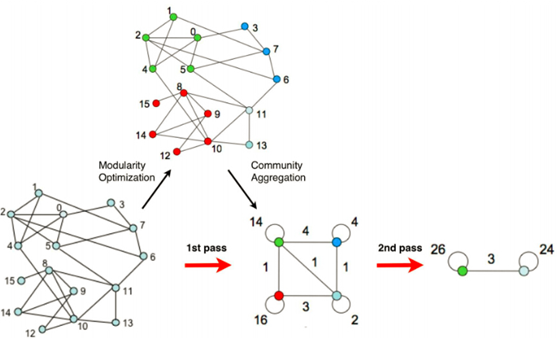
\includegraphics[width = \columnwidth]{2.png}
\caption{}
\end{figure}

We will illustrate the algorithm as following steps.

\begin{enumerate}
\def\labelenumi{\arabic{enumi}.}
\item
  Initialization

  Just make all the nodes belonging to different communities. That is,
  if we have N nodes, we have N communities initially.
\item
  Modularity Optimization

  For each node, try to divide each point into the community where its
  neighboring point is located, and calculate the degree of module at
  this point. Judging whether or not the modularity before and after the
  division is increased, if it is yes, then accept this division.
\item
  Community Aggregation

  This is the core of the algorithm. In this step, we will turn all the
  nodes in a same community into one new big node.
\item
  Iteration

  Iterate the algorithm until the directed graph does not change.
\end{enumerate}

Using such algorithms and all the methods above, we can get the Data Visualization result in Figure \ref{3} and Figure \ref{5}

\begin{figure}[ht]
\centering
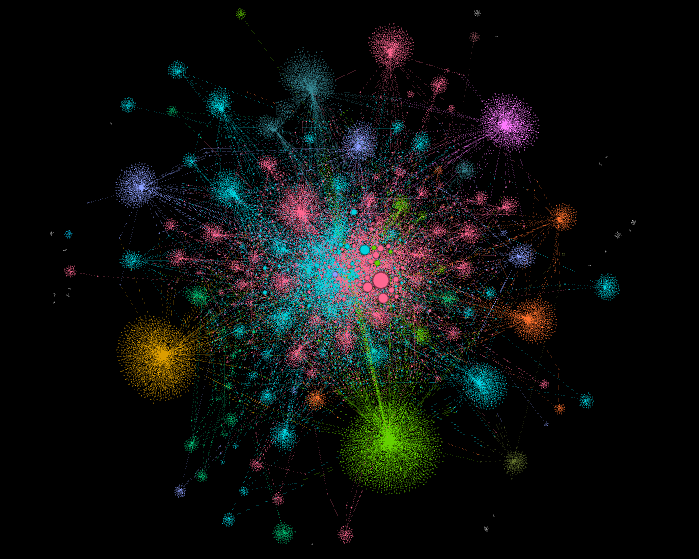
\includegraphics[width = \columnwidth]{3.png}
\caption{}
\label{3}
\end{figure}

\begin{figure}[ht]
\centering
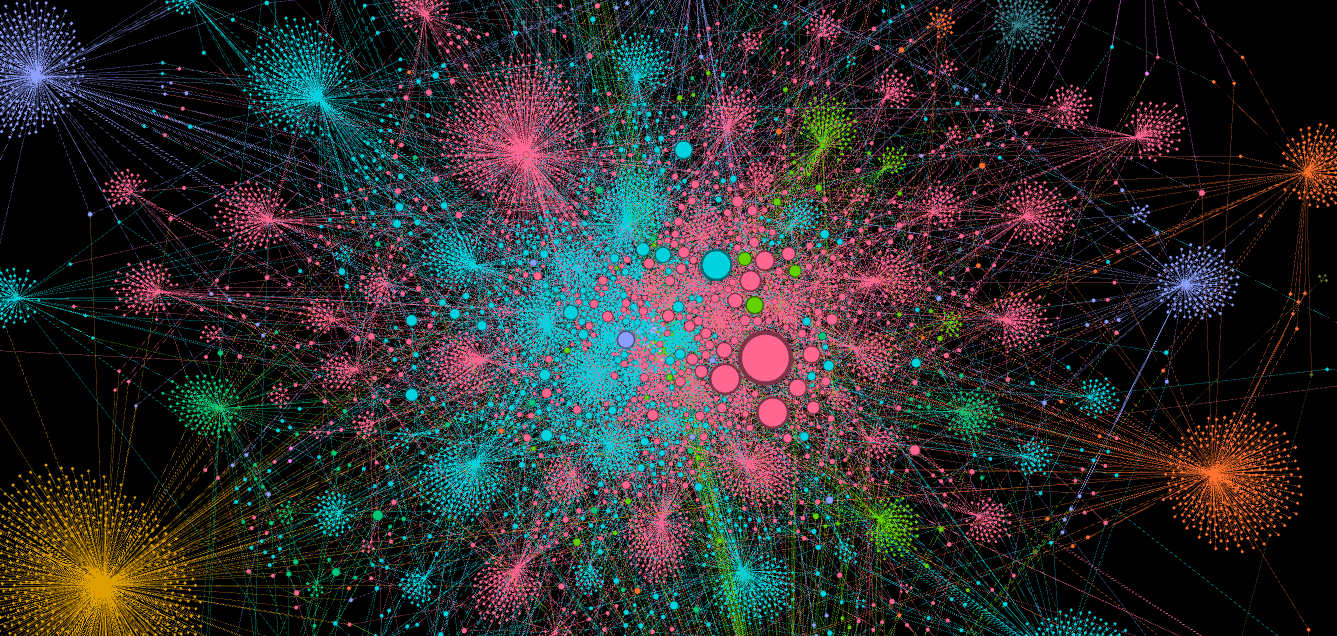
\includegraphics[width = \columnwidth]{5.png}
\caption{}
\label{5}
\end{figure}

Different colors denote different community. And we can know that the
biggest pink node in the middle has the most followers, (shown in Figure \ref{6})

\begin{figure}[ht]
\centering
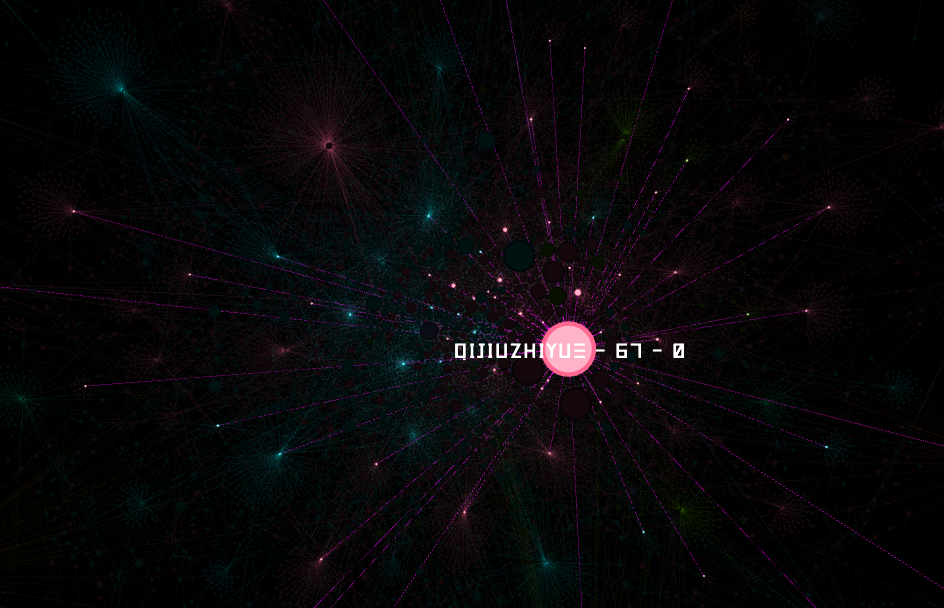
\includegraphics[width = \columnwidth]{6.png}
\caption{}
\label{6}
\end{figure}

Zoom in, we can find the user's information: user's ID, number of
followers and number of following. Besides, we highlight all the related
nodes for ease of observation. (shown in Figure \ref{4})

\begin{figure}[ht]
\centering
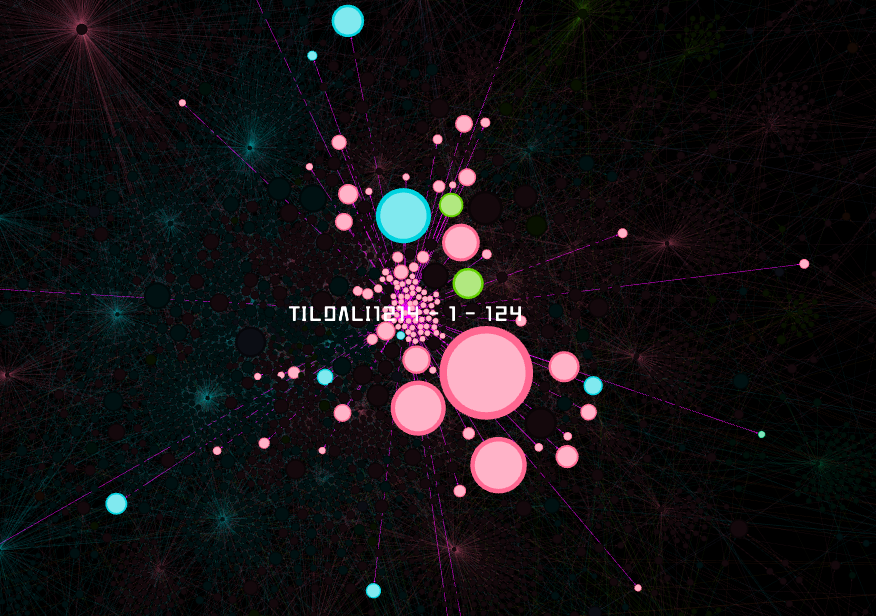
\includegraphics[width = \columnwidth]{4.png}
\caption{}
\label{4}
\end{figure}


\section{Collaborative Topic Regression}
In this section, we implement the collaborative topic regression
(CTR) model\citep{wang2011collaborative}. CTR combines traditional traditional collaborative
filtering with topic modeling. More specifically, it is a combination of Probabilistic Matrix Factorization (PMF) and Latent Dirichlet allocation (LDA). First, we get to know a bit about backgrounds of this model.

\subsection{Bachgrounds}
\paragraph{Recommendation by PMF}
Matrix Factorization is a simple but effective latent factor methods. We represent users and items in a shared
latent low-dimensional space of dimension $K$. User $i$ is represented by a latent factor $u_i$ while itme $j$ is represented by a latent factor $v_j$. The rating is then computed as

\[\hat{r}_{ij} = u_i^T v_j\]

The method is named matrix factorization, because Rating matrix $R$ is estimated by product of user matrix $U = {u_i}$ and item matrix $V = {v_j}$.
\[R=U^T V\]

PMF, as its name infered, brings in the idea of probability. The model assume the following generative process,

\begin{enumerate}
  \item For each user i, draw user latent vector $u_i \sim N(0,\lambda_u^{-1}I_K)$.
  \item For each item j, draw user latent vector $u_i \sim N(0,\lambda_v^{-1}I_K)$.
  \item For each user-item pair $(i,j)$, draw the response
  \[ r_{ij} \sim N(u_i^T v_j, c_{ij}^{-1})\]
  where $c_{ij}$ is the precision parameter for $r_{ij}$.
\end{enumerate}

Here $c_{ij}$ is a confidence parameter. If $c_{ij}$ is large, we trust $r_{ij}$ more, so we give real ratings higher value of $c_{ij}$.

\paragraph{Topic Models: LDA}
Topic models are a useful model in NLP. It is used to discover a set of "topics" from a large collection of documents. From one aspect, topic models provide an interpretable low-dimensional representation of the documents.

LDA is the simplest and most-frequently-used topic model. LDA assumes there are $K$ topic $\beta_{1:k}$ is a distribution over a fixed vocabulary. The model process is as follows:

\begin{enumerate}
  \item Draw topic proportions $\theta_j \sim Dirichlet(\alpha)$
  \item For each word ,
    \begin{itemize}
      \item Draw topic assignment $z_{jn}\sim Mult(\theta_j)$
      \item Draw word $w_{jn} \sim Mult(\beta_{z_{jn}})$
    \end{itemize}
\end{enumerate}

LDA models on document-theme distribution over word-theme distribution and learn the parameters $\alpha, \beta$ with EM algorithm.

\subsection{Model Introduction}
From the previous bachgrounds, we found that MF or PMF simply ignore the item information and thus, the learnt latent space cannot be interpreted. Also, it cannot genneralize to completely unrated items. A good way to solve these two drawback is to assign items with latent factors with meaning. A simple way is start with item content and extract valuable features.
The first approach is replacing the latent item factor $v_j$ with the its theme factor $\theta_j$ and generate ratings as,
\[r_{ij} \sim N(u_i^T \theta_j, c_{ij}^{-1})\]
but it cannot distinguish topics for explaining recommendations from topics important for explaining content.

Thus, we introduce collaborative topic regression (CTR). It represents users
with topic interests and assumes that documents are generated by
a topic model. CTR additionally includes a latent variable $\theta_j$ that
offsets the topic proportions $\epsilon_j$ when modeling the user ratings. Details will be illustrated in next section.

\subsection{Model Details}
The graphic model of CTR is shown in Figure \ref{ctr}. The generative process is as follows,
\begin{enumerate}
  \item For each user $i$, draw user latent vector $u_i\sim N(0,\lambda_u^{-1}I_K)$.
  \item For each item $j$,

  \begin{itemize}
    \item Draw topic proportions $\theta_j \sim Dirichlet(\alpha)$
    \item Draw item latent offset $\epsilon_j \sim N(0, \lambda_v^{-1} I_K)$ and set the item latent vector as $v_j = \epsilon_j+\theta_j$
    \item For each word $w_{jn}$,

      1. Draw topic assignment $z_{jn}\sim Mult(\theta)$

      2. Draw word $w_{jn}\sim Mult(\beta_{z_{jn}})$
  \end{itemize}
  \item For each user-item pair $(i,j)$, draw the rating
  \[r_{ij} \sim N(u_i^T v_j, c_{ij}^{-1})\]
\end{enumerate}

The key is how $v_j$ is generated. $v_j\sim N(\theta,\lambda_v^{-1}I_K)$.

\paragraph{Learning parameters}
The parameters are learned by EM algorithm to learn the maximum a posteriori (MAP) estimates.

\[u_i \Leftarrow (VC_iV^T+\lambda_u I_K)^{-1}VC_i R_i\]

\[v_i \Leftarrow (VC_jV^T+\lambda_vI_K)^{-1}(UC_jR_j+\lambda_v\theta_j)\]

and a good estimate of $\theta$ is the estimate from vanilla LDA.

After we estimate $U,V,\theta$, we can optimize $\beta$,

\[\beta_{kw}\propto\sum_j \sum_n \phi_{jnk}1[w_{jn}=w]\]
\begin{figure}
\centering
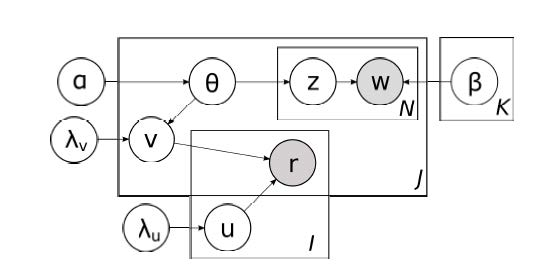
\includegraphics[width = \columnwidth]{ctr.jpg}
\caption{}
\label{ctr}
\end{figure}

\paragraph{Prediction}
After we have estimate of $U*, \theta*_{1:J} $and $\beta$. We will provide two ways to predict rating: in-matrix and out-matrix.

For in-matrix prediction which both user and item has record, we predict as
\[r_{ij}^* = (u_i^*)^T(\theta_j^*+\epsilon_j^*) = (u_i^*)^T v_j^*\]


For out-matrix prediction which item is new, we predict as
\[r_{ij}^* =  (u_i^*)^T \theta_j^*\]

\section{Experiments}
In experiment, we use the average rating $\bar{r}_ij$ of a movie and set $r_ij$ in the model to be the difference of user's rating and average rating $r-\bar{r}_ij$. This shows the user's own perferance and can give a more accurate estimate.

Because CTR takes huge computational cost, we only perform it on small dataset provided in the first time. We conduct 5-Fold Cross Validation.

Here we adopt same parameter setting in \citep{wang2011collaborative}, but the question is how to define a document for a item (movie).

In this Douban Movie Recommendation task, items are movies. Clearly, we cannot extract features through video. But, we can use item information provided by Douban and other DBPedia, like directors, actors, types, countries and so on. Moreover, we can go onestep further besides using tag-information listed above. Movie summaries mainly summarize the plot of the movie and contain lots of information about the movie. We produce several setting for three different document selection

\begin{itemize}
  \item all: 'title', 'directors', 'year', 'actors', 'type', 'countries', 'summary'
  \item summary: 'summary'
  \item other: title', 'directors', 'year', 'actors', 'type', 'countries'
\end{itemize}

The results is shown in Table \ref{tab:1}

% Table generated by Excel2LaTeX from sheet 'Sheet1'
\begin{table}[htbp]
  \centering
  \caption{Recommendation Results}
    \begin{tabular}{lrrr}
      \toprule
          & \multicolumn{1}{l}{all} & \multicolumn{1}{l}{summary} & \multicolumn{1}{l}{other} \\
          \midrule
    RMSE  & 0.9217 & 0.8790 & 0.8867 \\
    MAE	&0.7458&	0.7279&	0.7303\\
    \bottomrule
    \end{tabular}%
  \label{tab:1}%
\end{table}%

Surprisingly, CTR with all information performs worst among three.

Here we extract top-10 words from certain generated topics and it shows that our topic model give explicit split to different kinds of movies.

We provide an example for top-10 words in certain topic, and we can see it is effective.

\begin{figure*}[ht]
\centering
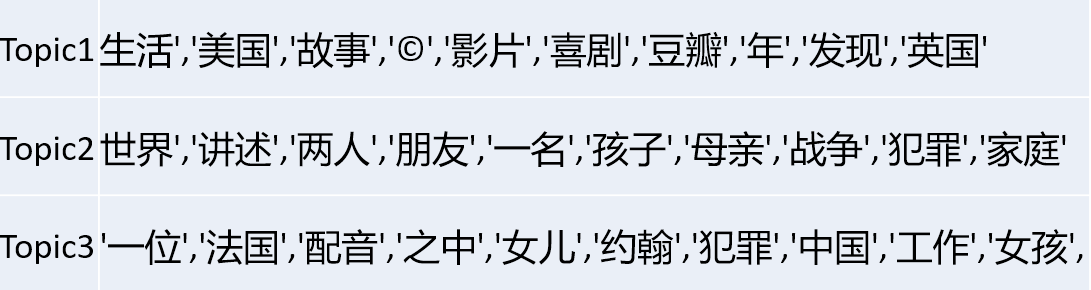
\includegraphics[width = 10cm]{7.png}
\caption{}
\label{7}
\end{figure*}

\begin{figure*}[ht]
\centering
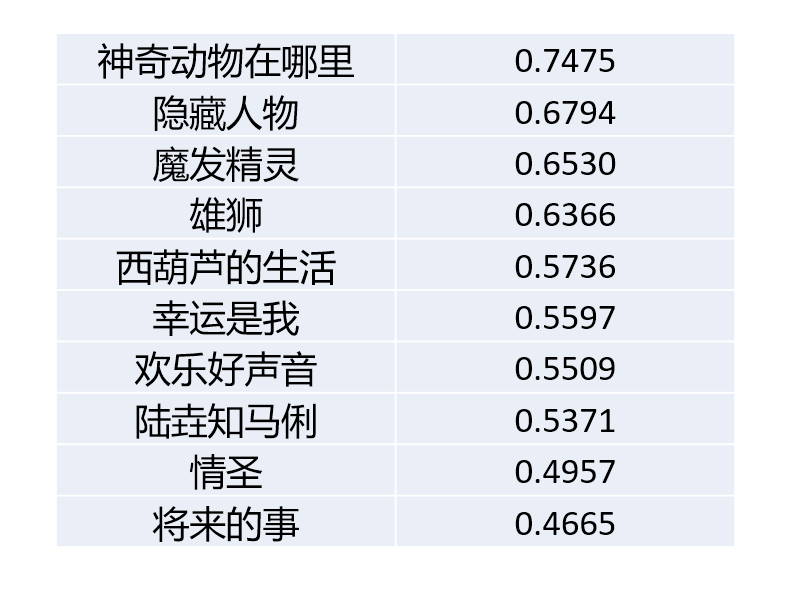
\includegraphics[width = 10cm]{8.png}
\caption{Example of recommendation via preference}
\label{}
\end{figure*}

\begin{figure*}[ht]
\centering
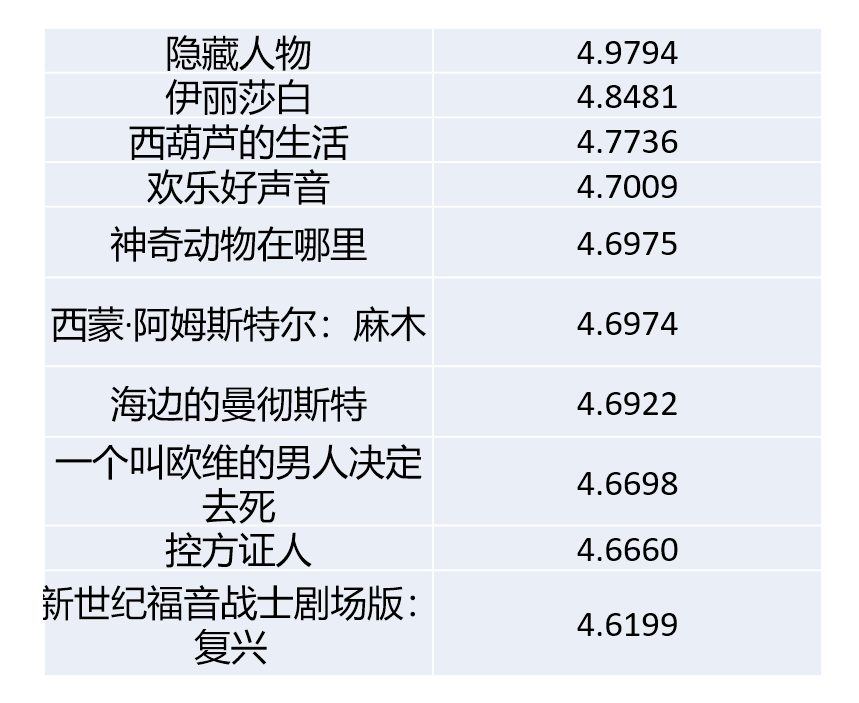
\includegraphics[width = 10cm]{9.png}
\caption{Example of recommendation via overall rating}
\label{}
\end{figure*}


\hypertarget{header-n72}{%
\section{Another Idea of Feature Extraction}\label{header-n72}}

The basis of the content-based recommendation system is that the user's
interests should match the description of the system's recommended
items. In other words, the more similar the user's interest is to the
description of the item, the more interested the user may be in the
recommended item. The content-based recommendation system achieves this
by measuring the similarity between the description of a project and the
user's personal information. The higher the similarity, the greater the
chance of the project being recommended.

We use some algorithms to embed the information of the movie and the
user's information in the same semantic space.

\hypertarget{header-n77}{%
\subsection{Movie Information Embedding}\label{header-n77}}

Specifically, the embedded movie vector consists of provided movie
information. We have adopted information including the movie's
publication time, ratings, screenwriters, directors, and actors.

In particular, in this project, \textbf{we proposed an original method
of embedding actors and directors in Low-dimensional vector space.} We
label both the director and the actor as artists, build an adjacency
matrix from the number of movies they have worked with, and then use the
SVD matrix decomposition to get a low-end matrix. This method not only
greatly reduces the dimension, facilitates subsequent calculations, but
also has certain semantic information embedded, which is a more reliable
method.

As the saying goes, things are gathered together and people are divided
into groups. We know that often-co-directed directors and actors may
have similar film styles. For example, the actors often appearing in
Qiong Yao's TV series may have similar artistic styles and they all like
to play soap operas. And the audience may be similar to their
preferences.

\textbf{This algorithm's inspiration comes from the word2vec algorithm.}
In the word2vec algorithm, semantically similar words are closer in
semantic space. Considering the following sentences:

\begin{itemize}
\item
  The tiny \textbf{} is so cute!
\end{itemize}

We will easily think of cat, puppy, dog, etc according to semantic
environment. And it can be proved as the Bing search result as below.

\begin{figure}
\centering
\includegraphics[width=\columnwidth]{11.png}
\caption{}
\end{figure}

So in the movie situation, considering the following artists:

\begin{itemize}
\item
  Tim Burton, Johnny Deep,
\item
  Daniel Radcliffe, Alan Rickman, JK Rowling.
\item
  Fan Bingbing,Zhao Wei,Su Youpeng
\end{itemize}

You might think of Helena Bonham Carter, Emma Watson, Lin Xinru
respectively. And you will never think of a Chinese actor in the first
movie environment just like you will never think of a word like
''bottle'' in the ''The tiny XXX is so cute!'' semantic environment.
Then environment entails the information! Therefore, in word2vec
algorithm, we will use the words around a particular word as the
"environment" to train the word embedding model. And in the "movie
environment", we believe the co-operation entails the environment. We
will build a "Co-operation matrix" \(M\) like below.

\begin{longtable}[]{@{}llll@{}}
\toprule
Co-operation Matrix & Tim Burton & Johnny Deep & Helena
Carter\tabularnewline
\midrule
\endhead
Tim Burton & 16 & 9 & 7\tabularnewline
Johnny Deep & 9 & 17 & 8\tabularnewline
Helena Carter & 7 & 8 & 15\tabularnewline
\bottomrule
\end{longtable}

If we have 10000 artists in total, we can have a such 10000 *10000
dimension "Co-operation matrix". And then we can SVD the matrix:

\[M = U\times S\times V\]

We will choose the top n (here 100) important dimension of all U,S,V
matrix to get off the noise as the figure shows. We denote them as
\(U',S',V'\) respectively. We will rebuild the M matrix.

\[U'\times S'\times V' = M'\]

In this situation, each \textbf{artist can be represented by a
100-dimension vector.}

\[v_{artist_{i}} = M'_{row_{i}}\]

And finally, we have

\[v_{movie_i} = cat(v_{artist_i},v_{rating_i}, v_{date_i},...)\]

In the experiment, we selected all actors (about 2,000) who performed
more than 8 times in 10,000 movies and established such a ``cooperation
matrix'' and then reduced it to 100 dimensions through PCA. This gives
each artist's expression. Finally, we use the TSNE algorithm to reduce
the matrix to 2 dimensions and visualize it. As can be seen in the
figure below, like the semantic space of word2vec, the low-dimensional
representation of our cooperation matrix dimension reduction can indeed
express a good cooperation relationship.

\begin{figure}
\centering
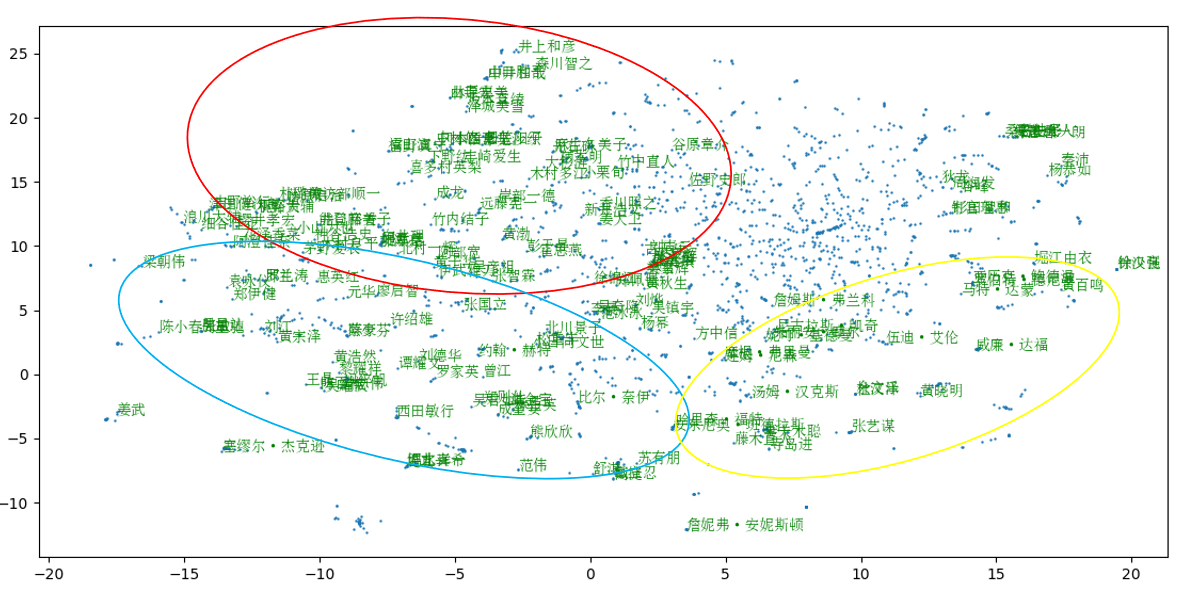
\includegraphics[width=\columnwidth]{10.png}
\caption{}
\end{figure}

As shown in the figure, the red region is basically a Japanese artists
community, the blue region is for Chinese artists, and the yellow one is
mainly a European and American region.

\hypertarget{header-n152}{%
\subsection{User Information Embedding}\label{header-n152}}

For every user, we have their rating information. We can suppose that
they love those movies which they rate them as 5 score. So we can use
all the movies they love to represent them. In this situation, we will
denote the user embedding vector as the average of their 5-score movies'
embedding vector.

\[v_{user} = \dfrac{1}{n}\sum v_{movie_{5-score}}\]

We can use this method to build the users' denoting.

% Bibliography
\bibliography{biblio}
\bibliographystyle{acl_natbib}


\end{document}
